% Options for packages loaded elsewhere
\PassOptionsToPackage{unicode}{hyperref}
\PassOptionsToPackage{hyphens}{url}
%
\documentclass[
  openany]{book}
\usepackage{amsmath,amssymb}
\usepackage{iftex}
\ifPDFTeX
  \usepackage[T1]{fontenc}
  \usepackage[utf8]{inputenc}
  \usepackage{textcomp} % provide euro and other symbols
\else % if luatex or xetex
  \usepackage{unicode-math} % this also loads fontspec
  \defaultfontfeatures{Scale=MatchLowercase}
  \defaultfontfeatures[\rmfamily]{Ligatures=TeX,Scale=1}
\fi
\usepackage{lmodern}
\ifPDFTeX\else
  % xetex/luatex font selection
\fi
% Use upquote if available, for straight quotes in verbatim environments
\IfFileExists{upquote.sty}{\usepackage{upquote}}{}
\IfFileExists{microtype.sty}{% use microtype if available
  \usepackage[]{microtype}
  \UseMicrotypeSet[protrusion]{basicmath} % disable protrusion for tt fonts
}{}
\makeatletter
\@ifundefined{KOMAClassName}{% if non-KOMA class
  \IfFileExists{parskip.sty}{%
    \usepackage{parskip}
  }{% else
    \setlength{\parindent}{0pt}
    \setlength{\parskip}{6pt plus 2pt minus 1pt}}
}{% if KOMA class
  \KOMAoptions{parskip=half}}
\makeatother
\usepackage{xcolor}
\usepackage{longtable,booktabs,array}
\usepackage{calc} % for calculating minipage widths
% Correct order of tables after \paragraph or \subparagraph
\usepackage{etoolbox}
\makeatletter
\patchcmd\longtable{\par}{\if@noskipsec\mbox{}\fi\par}{}{}
\makeatother
% Allow footnotes in longtable head/foot
\IfFileExists{footnotehyper.sty}{\usepackage{footnotehyper}}{\usepackage{footnote}}
\makesavenoteenv{longtable}
\usepackage{graphicx}
\makeatletter
\newsavebox\pandoc@box
\newcommand*\pandocbounded[1]{% scales image to fit in text height/width
  \sbox\pandoc@box{#1}%
  \Gscale@div\@tempa{\textheight}{\dimexpr\ht\pandoc@box+\dp\pandoc@box\relax}%
  \Gscale@div\@tempb{\linewidth}{\wd\pandoc@box}%
  \ifdim\@tempb\p@<\@tempa\p@\let\@tempa\@tempb\fi% select the smaller of both
  \ifdim\@tempa\p@<\p@\scalebox{\@tempa}{\usebox\pandoc@box}%
  \else\usebox{\pandoc@box}%
  \fi%
}
% Set default figure placement to htbp
\def\fps@figure{htbp}
\makeatother
\setlength{\emergencystretch}{3em} % prevent overfull lines
\providecommand{\tightlist}{%
  \setlength{\itemsep}{0pt}\setlength{\parskip}{0pt}}
\setcounter{secnumdepth}{5}
\usepackage{booktabs}
\pagestyle{plain}
\renewcommand{\familydefault}{\sfdefault}
\usepackage[a4paper, margin=1in]{geometry}
\usepackage[]{natbib}
\bibliographystyle{plainnat}
\usepackage{bookmark}
\IfFileExists{xurl.sty}{\usepackage{xurl}}{} % add URL line breaks if available
\urlstyle{same}
\hypersetup{
  pdftitle={QuitUSM},
  pdfauthor={Mohamed Lashuel},
  hidelinks,
  pdfcreator={LaTeX via pandoc}}

\title{QuitUSM}
\author{Mohamed Lashuel}
\date{2025-08-12}

\begin{document}
\maketitle

{
\setcounter{tocdepth}{1}
\tableofcontents
}
\chapter{Introduction}\label{introduction}

This is a guide on how to quit unhealthy social media (USM), condensed from multiple books on addiction as well as inspired by my own experience. I use the term USM because I believe that social media platforms are not 100\% bad when used in specific ways. Social media use is USM if, for, example:

\begin{itemize}
\tightlist
\item
  You want to quit it, but can't
\item
  You use it much more than you intend to
\item
  You obsess over it while you're not using it
\item
  You find it difficult to be without it
\item
  It gets in the way of real life
\end{itemize}

This is in contrast to healthy social media use, which enriches your life, by e.g.~allowing you to connect with loved ones who are physically far away.

The intended audience is anyone who wants to cut down or quit their USM use, from someone who uses it ``only'' half an hour per day to heavy users who use it most of the day. The book is written as if you're a moderate to heavy user, but the principles should work for everyone.

I myself was addicted to video games and USM for years. Like many, I made attempts to cut down or quit, but failed every time. I feared I was chained to USM for life and even if I did quit I would slip back down eventually. I looked down on myself for not having enough willpower to stop. Today I am completely free from USM and video game addiction. I didn't do it with incredible self-control or with the encouragement of friends and family - it was a matter of reading the right ideas and coming to the right realizations at the right time. I learned that addiction is not a problem of having enough willpower, but a fiendish puzzle - frustratingly hard to solve on your own, but if you know the answer, it becomes trivial. I wrote this guide to share the answer to the puzzle with as many people as possible, because I believe that anyone can not only quit USM but be FREE. I say this as someone who went through the worst of it and knows the shame, self-doubt, and fear caused by being addicted.

When I say ``addicted'' I don't mean to scare you or bring up images of drug abusers who would do anything for a fix. The fact is that USM is inherently physically addictive, in that as you use it you need more and more to get the same result, and you experience withdrawals and cravings when you are not using it. Most Americans are physically addicted to USM, many without realizing. Don't worry, the fact that you're addicted won't make it any harder to quit. In fact, it will be slightly easier now because you're closer to solving the puzzle.

This guide is more like a set of notes than a book. If you skim, there's a good chance you miss an important point and don't understand the message. If concepts don't stick or you're confused, reread sections. Refer back to the guide if you're having trouble - it's definitely possible you forgot something. Take notes on the most important or most impactful points.

I'd wish you good luck, but you won't need it.

This book can be downloaded as a \href{main.pdf}{PDF} or \href{main.epub}{EPUB} file.

QuitUSM by Mohamed Lashuel is licensed under \href{https://creativecommons.org/licenses/by/4.0/}{CC-BY 4.0}.

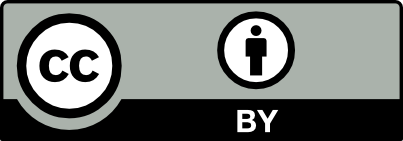
\includegraphics[width=0in,height=\textheight,keepaspectratio]{images/cc.png}

This website's code is open source and hosted on Github \href{https://github.com/MohamedLashuel/QuitUSM/}{here} licensed under the \href{https://github.com/MohamedLashuel/QuitUSM/blob/main/LICENSE}{MIT License}.

\chapter{Addictive aspects}\label{why-addictive}

Throughout this book I will refer to two different types of social media use:

\begin{itemize}
\tightlist
\item
  \emph{Personal}: Using social media to view and share content with family, friends, or acquaintances.
\item
  \emph{Impersonal}: Using social media to view content from people you don't know.
\end{itemize}

Your text messaging app is purely personal. YouTube and TikTok are examples of mostly impersonal apps, where most who use them just go through recommended videos. Most social media sites have both personal and impersonal elements. Facebook and Instagram were created to be primarily personal but will now shove onto your feed recommended posts from complete strangers.

\section{Why is social media addictive?}\label{why-is-social-media-addictive}

\subsection{Dopamine}\label{dopamine}

The main mechanism making social media addictive is dopamine. Dopamine is a chemical in the brain that is released when anticipating a reward. It reinforces and makes us repeat behaviors - if you eat a cookie (which releases dopamine) and find it pleasurable, you are likely to eat more. Sweet foods such as fruits were rare and valuable in prehistoric times, so our brains evolved to release dopamine in reaction to sugar, to encourage us to eat more of them. But in today's age, we have an unlimited supply of foods sweeter than anything natural, and many overconsume as a result. Social media also hijacks our natural rewards in the same way:

\begin{itemize}
\tightlist
\item
  \textbf{We seek out and are rewarded for social connections.} Personal social media keeps us constantly in the loop about friends and family and also lets us talk to millions of strangers across the globe. We also receive feedback from them in the form of ``likes''/``dislikes''. In fact, studies have shown higher social media use to be connected with higher levels of loneliness time and time again.
\item
  We are rewarded for finding information and novelty. When scrolling through social media posts or short videos, we are bombarding our brains with information and ``new'' things. This applies more to impersonal social media which can supply an endless stream of posts.
\item
  Social media uses a variable reward scheme rather than a fixed reward scheme. This is the same principle that a slot machine uses. While you're scrolling through videos, whether you find a funny one and are entertained is random. Or when you make a post, you can't predict if it will blow up and get you many likes/good comments. Random rewards are much more addictive than predictable rewards. Imagine how less entertaining a slot machine would be if it simply rewarded you every 3rd spin instead of randomly.
\end{itemize}

USM use is the digital equivalent of junk food, releasing an amount of dopamine our brains were not equipped to handle on a daily basis. When an unnaturally high amount of dopamine is being released, the brain has a self-correcting mechanism to trim down the number of dopamine receptors. The brain now receives less dopamine which brings rewards down from USM to normal levels. Unfortunately, it also decreases rewards from all other activities. Actions such as eating or talking to friends feel less satisfying while an increasing amount of USM use is needed to get that same ``high'' (which is actually a normal level of dopamine). Without USM, the user starts to feel withdrawals. This process is called dopamine desensitization.

If you are affected by dopamine desensitization, you have normal levels of dopamine when using USM and low levels at all other times. Compare to a non-user who has normal levels at some times and high levels at others.

The physical effect of withdrawals is lowered dopamine levels in the brain. This results in a low mood, lack of pleasure from normal activities, boredom, and/or low motivation. If you watch YouTube for 5 hours, by the end you have no drive to accomplish anything and everything feels less enjoyable. USM addicts often suffer from anhedonia (loss of pleasure in normal activities) and find it difficult to muster the energy to work.

Fortunately, the brain is able to recover from desensitization in a matter of weeks, with physical withdrawals diminishing then disappearing, if the source of unnaturally high dopamine (USM in our case) is removed.

\subsection{Intentional Design}\label{intentional-design}

All popular social media apps are free. They make income by showing advertisements to their users. These apps collect data on what you do in their apps, which posts you watch or like, what you search for, which communities you visit, etc. They do two things with this information:

\begin{itemize}
\tightlist
\item
  Feed it to their algorithms in order to determine which content to recommend to you. For example, as you use YouTube more, it will learn which videos you like watching, and the videos you get recommended will be more and more likely to draw your interest. The goal is to maximize the time you spend in their app to show you more advertisements.
\item
  Serve you targeted ads based on your predicted demographics, location, and interests. With the personalized data they have, your attention becomes especially valuable to advertisers who are willing to pay more to show their ads to the exact type of customer they want.
\end{itemize}

Again, the more time you spend on their apps, the more data they collect and the more advertisements they can show you. Thus, they have an incentive to keep you on their apps for as much time as possible. Features like infinite scrolling and autoplay seek to make using their apps as frictionless as possible so you spend more time on them without realizing it. They also love to send you notifications, because each time you click on them and open the app is more time spent.

A common saying is ``If a service is free, you are the product''.

\section{Other factors}\label{other-factors}

\begin{itemize}
\tightlist
\item
  \emph{Availability}: For most of us, our phones are with us 24/7, with social media apps taking only a few seconds to access. This makes it easy to act on impulses and build habits of opening them. It also naturally fills up our downtime, such as if we're waiting at a bus stop.
\item
  \emph{Fear of missing out (FOMO)} (Personal social media): Humans hate being excluded socially. When putting down, for example, Facebook or Instagram, we worry about missing out on friends' activities. We also like being ``in the loop'' on current events and trends. It feels uncomfortable to not have access to this information if we are used to it.
\item
  \emph{Normalcy}: Anything that society accepts and views as normal will be more easily acceptable to me or you. In other words, ``It's okay if everyone does it''. On the other side, people fear sticking out by not using social media.
\end{itemize}

\section{The addiction trap}\label{the-addiction-trap}

Even though users know all the trouble USM causes, the wasted time, loss of sleep, etc., they actually dread and fear the idea of quitting. They see USM as a crutch or vice which would cause them great pain to give up. Users are torn between wanting to keep using and wanting to quit. Remaining addicted looks like the lesser of two evils, so they choose to keep using rather than quit. This is the addiction trap. Try to understand this in your own experience of USM use: you may recognize that quitting would be better and healthier for you (which I assume is true if you are reading this guide), but at the same time you WANT to pick up the phone to use USM. When you think of quitting, are you excited at the prospect of freedom, or get a feeling of anxiety?

Addiction is suffering, but to addicts it looks like the lesser of two evils.

From an outsider's perspective, it's easy to see that, for example, a heavy smoker really would be better off if he gave up smoking. After all, it causes numerous health issues, costs a lot of money, and for what benefit? The smoker, however, can't see it this way because he is inside the trap. USM addicts are likewise fooled by the trap into thinking that USM is a genuine pleasure or benefit, or that they would suffer a great loss if they gave it up.

\chapter{The two monsters}\label{two-monsters}

\section{The little monster}\label{the-little-monster}

In Chapter \ref{dopamine} I went over dopamine. The main reason we use USM is to end dopamine withdrawal and feed the ``little monster''. The little monster awakens when we go through dopamine withdrawal. Whenever you have free time, it feels like something is missing. You feel empty or restless - this is the little monster begging to be fed. If we give in to it, we are satisfied momentarily, but once we put down USM, dopamine levels start to decrease, starting the cycle over again.

Dopamine withdrawal is caused by USM use, not relieved by it. No non-user ever went through USM withdrawal.

If you abstain from USM for long enough, as your dopamine baseline returns to normal, the little monster will grow weaker and weaker before eventually dying out. The empty feeling disappears along with the other symptoms of withdrawals (low mood, lack of motivation and pleasure).

By itself, the little monster is a minor threat and if this was all there was to it, quitting would be easy.

\section{The big monster}\label{the-big-monster}

Much more dangerous than the little monster is the big monster. Remember that all addicts are pulled in two directions, wanting to quit and wanting to use. The big monster is the part of you that wants to use. It comes from the (false) belief that USM gives you genuine pleasure or benefit. Once you understand it, there is no reason to want to use USM anymore.

You may have heard of smokers who have quit for years, then pick up one cigarette and are hooked again. You may also have heard of alcoholics who quit drinking but have been miserable without alcohol since then. They defeated the little monster long ago, but failing to address the big monster, they eventually chose the pleasure of the drug - a pleasure that doesn't actually exist. Setting off the little monster, they fell back into the trap of addiction.

\subsection{The illusion of pleasure}\label{the-illusion-of-pleasure}

I mentioned that USM users are fooled into thinking thinking that there is a genuine pleasure to USM. This can be attributed to the dopamine release that USM causes. Remember that as you use more and more, dopamine desensitization occurs in the brain. You go through your life with lowered dopamine levels experiencing withdrawal most of the time and need to use USM to return to normal levels. Non-users don't get withdrawals, and the relief you get from using USM is what they feel all the time. In other words, you use USM to feel like someone who doesn't. Clearly you would have been better off if you hadn't become hooked in the first place. All you need to do is to stop using USM and your dopamine levels will return to normal.

You may be thinking ``I know that already'' but it probably hasn't truly sunk in. The problem is that the facts don't fit in with a user's experience. It is when you are using USM that you feel normal, and when you are not using, you suffer from withdrawal. When you feel low and empty, as soon as you pick up USM, your problem is cured. Your brain makes the obvious connection: using social media makes you feel better, not using it makes you feel bad, therefore it must be a good thing. This is the opposite of the truth - whenever you stop USM you feel bored, or empty, or depressed, but this is caused itself by using USM. Addicts think that their problems will be solved by the next hit of their drug, but in reality they were caused by the previous hit - an endless cycle until you break out.

Using USM is like wearing tight shoes all day to get the ``pleasure'' of taking them off. Taking the shoes off is a relief, but only from the pain it causes.

Think of the absolute misery heroin addicts go through when they are deprived of their drug. Now think of the utter joy they get when they are finally able to stick a needle in their veins and end their cravings. Non-heroin addicts don't get that feeling of joy - it's caused by the little monster. We don't see it this way because the process of building tolerance to dopamine is slow and gradual. If the instant you used USM for the first time, you became hooked, becoming restless without it and needing to use it for hours to get through the day, it would quickly register that USM was the problem. In reality, withdrawals are slight as we begin to use, so we don't blame USM. By the time we realize we need to cut down, USM has cemented its place in our mind as something to reach for when we need a boost, to relax, or whenever we're bored and it doesn't occur to us the problems it fixes are the very ones it causes.

Another contributor to the illusion is other people. Since all other USM addicts are also in the trap, they also fall for the illusion and report that they want to quit USM, but it's just \emph{so enjoyable}. This has a profound impact on your subconscious when repeated. The effect is to accept without taking for granted the pleasure of USM. Whenever you hear anything to this effect, take note the ``enjoyment'' is just the removal of the withdrawal.

\chapter{The ``benefits'' of social media}\label{benefits}

At this point, even if you recognize that USM doesn't give you real pleasure, you may have in mind some other benefit it gives you. The supposed ``benefits'' generally are the same case as the illusion of pleasure, where USM causes the symptom that it temporarily relieves.

Another type of ``benefit'' is the excuse. I define an excuse as anything used to justify USM use but isn't the real reason they use USM. To use an analogy, smokers may say they smoke because they enjoy their particular brand of cigarettes. In reality if their preferred brand wasn't available, they would still smoke whatever was on hand. The most important reason we use USM is to feed the little monster, but users feel uncomfortable with that idea and find the excuses much easier to swallow. It doesn't help that everyone else is also using excuses and so we give them more validity in our minds. This process is only semi-conscious and often addicts don't know they're doing it, so whatever benefit you see in USM, try to interrogate it. Would you still use USM without that benefit? If so, it's an excuse.

If you rationally weighed up the costs and benefits of using, the costs would win ten times over.

\section{Relieving boredom}\label{relieving-boredom}

USM causes boredom itself. Remember that boredom is a symptom of dopamine withdrawal, and the high dopamine levels brought by USM cause said withdrawals. USM users are more bored in their day-to-day lives than non-users - It's only when they are using USM they can get rid of that boredom. For this reason, USM users find it harder to get work done or do chores.

Caveat: USM does relieve boredom in that if you are bored and you choose to use it, then you will be less bored while you are using it. But by using USM to kill time instead of anything fun, meaningful, or productive, you are wasting time and keeping the cycle of boredom going, since USM also causes boredom. And what do you get out of it? Once you're done you feel worse than when you started.

Many trying to quit USM report feeling something like a ``void'' in the first few days. If you have been overstimulating your brain with USM during every bit of downtime, it will take a little time to adapt to having that stimulation taken away.

\section{Relaxation}\label{relaxation}

USM users state that it helps them relax or unwind. I will frame this in a different way: USM users find it difficult or impossible to relax while doing nothing, so they must have USM to relax. As long as you believe the big monster, the little monster's nagging makes it uncomfortable to be alone with your thoughts, so users can't relax as well as non-users in a situation such as sitting on a park bench on a nice day or putting your feet up after getting home from work.

\section{Concentration}\label{concentration}

Users know that USM can be extremely disruptive to focus. How often does just checking a notification turn into a wasted half hour while you should be doing work? At the same time, those who try to quit often have troubles concentrating on tasks. This is due to dopamine withdrawal causing boredom and low motivation and the distractions of the little and big monster. You get a craving and the big monster starts pestering you to let go of your work and use USM instead. Once you've defeated the big monster, your concentration restores to normal levels.

\section{Dealing with negative emotions}\label{dealing-with-negative-emotions}

Stress, sadness, and anxiety are often caused by USM itself. There's the shame of having wasted hours, fear of missing out, the stress of deadlines after procrastinating with USM, etc. Even if we disregard that, is USM really a good way to deal with these emotions? It distracts you in the moment, but once you're done using, the emotions are still there. In fact, they've probably compounded.

\section{Social connections}\label{social-connections}

Remember from Chapter \ref{dopamine} that our brain rewards us for building social connections. Social media games this by providing us many more social connections than in the real world at the cost of not being as fulfilling. Does it really matter how many complete strangers from across the country or friends of friends of friends ``like'' your post or comment? No, the point is to feed your little monster.

I will throw personal social media a bone and say it CAN be used for authentic social connection if used very carefully. I don't think there's anything wrong with posting family pictures for close friends to see. Lots of people who text or call their friends do it on social media apps, so if you use those apps just to text or call them, I would say it's a good use. The problem is that social media can replace real-world interactions. The benefit from browsing friends' posts is nowhere near that of having a cup of coffee with them. Plus, the more time you spend on USM in general, the less time that leaves for real-world interactions.

\section{Entertainment}\label{entertainment}

This mainly applies to impersonal social media. The idea that USM is more entertaining than, say, watching a movie is essentially a symptom of withdrawals. Heavy users don't get as much enjoyment out of watching a movie because of dopamine withdrawal. They are physically more bored and have a restless feeling, like they'd love to be using USM instead. USM may be entertaining at first, but as your tolerance increases it becomes less and less so.

Perhaps you can point to specific YouTube channels or comics you follow as real entertainment. Perhaps, but then why scroll through infinite feeds of recommended posts on these apps?

\section{Information}\label{information}

Social media does have plenty of useful information, but this is not by itself a reason to use USM since said information is almost always found easier and faster elsewhere, without any of the downsides or major distraction provided by USM.

Some enjoy learning fun facts or trivia through their USM feeds. In the same vein as entertainment, a long article or book can't compete with the dopamine release from USM in terms of interest. The article is plenty interesting in the eyes of a non-user.

\section{Keeping up}\label{keeping-up}

On the personal side, there is keeping up with friends' and colleagues' social media posts. Maybe you can argue that it's a benefit to be aware of, for example, events that happen in your city which are posted on social media, which I would agree with, but the desire to keep up can quickly become the fear of missing out (FOMO). This is provoked by USM - those who don't use it don't need to check it daily to not feel like they're missing out. A modern proverb goes, ``After one day without social media, I feel like I missed everything; after one month, I feel like I missed nothing''. Examine whether you are actually getting useful information and keeping in touch with loved ones or just keeping up for the sake of keeping up.

On the impersonal side, there is keeping up with news and politics. If you're looking at reputable news organizations that happen to have pages on social media, fair enough. But getting information from regular users is risky at best. Without any regulation, misinformation is abundant on social media. A study from \emph{Science} indicates that fake news spreads 6 times faster than real news because it is more emotionally charged and more attention-grabbing\footnote{\url{https://science.sciencemag.org/content/359/6380/1146.full}}. An Oxford University study of 22 million political tweets in 2017 found users shared more ``misinformation, polarizing, and conspiratorial content'' than actual news\footnote{\url{https://www.researchgate.net/publication/323142063_Social_Media_News_and_Political_Information_during_the_US_Election_Was_Polarizing_Content_Concentrated_in_Swing_States}}. Don't think it's so easy to tell which is which - sure, if it seems outrageously wrong you can tell, but what about misinformation which you agree with? When you read a fact or statistic that confirms what you already thought, do you go out of your way to check it?

If you think social media is good for political content, here is an experiment you can try. Seek out a political group on social media that opposes your beliefs. If you read through them, you will probably notice lots of misinformation and nonsensical points. People tend to believe almost anything if it's repeated over and over among people they know, like, or see common ground with. Over time, this creates an ``echo chamber'', where false facts are never challenged and keep growing. What is happening to these people is also happening to you, it doesn't matter how ``rational'' you think you are. All users on social media are exposed to staggering amounts of fake news, and since nobody fact-checks every single thing they read this inevitably turns into false beliefs. Garbage in, garbage out. Here's one more study: Researchers from Carnegie Mellon judged 45\% of tweets about the coronavirus in early 2020 to be likely written by bots contributing to over 100 false narratives.\footnote{\url{https://www.kpbs.org/news/2020/may/20/researchers-nearly-half-of-accounts-tweeting/}}

Each side thinks they are perfectly logical and obviously correct while the other side is crazy.

\section{The benefits of quitting}\label{the-benefits-of-quitting}

Addicts dealing with the big monster despair at the thought of quitting. I would like to emphasize the benefits of quitting in order to cement the idea that quitting is the happier option for you, compared to staying addicted to USM. Don't skim through this list! Read each item carefully and envision the benefit of each one.

\begin{itemize}
\tightlist
\item
  No cravings from the little monster
\item
  Reclaiming all the time you spend on USM
\item
  Not being distracted by USM while trying to work, or procrastinating with USM
\item
  Better attention span
\item
  No dopamine withdrawal (better mood, less boredom, more motivation)
\item
  Not losing sleep late at night to USM
\item
  No shame from being addicted
\item
  No fear of being hooked for life
\item
  Being able to enjoy the moment without USM at hand
\item
  No longer comparing yourself to strangers online
\item
  Less tiredness
\end{itemize}

\chapter{Difficulties in quitting}\label{difficulties-in-quitting}

How do you quit a job? It's sort of a silly question. You say ``I quit'' and you never go back to the job again. With USM, it's easy to say ``I quit'' but the trouble lies in making sure you don't return.

\section{The willpower method}\label{the-willpower-method}

As stated previously, addicts both want to keep using and want to quit. The typical approach to quitting is to not address the desire to keep using and try to brute force it with willpower. If you are trying to resist your desire to use USM day in and day out with willpower alone, that is very difficult for a few reasons:

\begin{itemize}
\tightlist
\item
  You are constantly straining at the leash to fight against doing the very thing you want to do
\item
  This stress is doubled without being able to turn to USM, which addicts are dependent on to deal with stress
\item
  As you recover from addiction and withdrawal symptoms fade, the reasons you had for quitting start to disappear, and the want to use becomes stronger compared to the want to quit
\item
  If you give in, it doesn't satisfy your cravings. Instead you want to use more and it is easy to fall back into your old ways
\item
  USM appears more precious, like dieting makes unhealthy food more tempting
\end{itemize}

The hope is that if you can go long enough without using USM, the desire to use it will go away. This does work for many people, it sinks in that life is better without USM and the former addict can live freely. But overall, the rate of failure is high for the reasons I listed above. Even if one succeeds, since they haven't beaten the big monster they might be pining to use USM long after they kicked the physical addiction.

Quitting with willpower is hard because you are trying to not do something you desparately want to do.

\section{The fear of quitting}\label{the-fear-of-quitting}

USM users are afraid to quit because they believe they are losing a crutch or genuine pleasure (believing the big monster). They fear that the emptiness and boredom they feel when not using USM will be with them forever (not understanding dopamine desensitization). They despair at the thought of never getting the pleasure of using USM again (the illusion of pleasure). By now you should realize that all of these feelings are irrational. There is also the fear of withdrawals and cravings which I have yet to address.

\subsection{Withdrawals and cravings}\label{withdrawals-and-cravings}

We already went over the physical effects of dopamine withdrawal: low mood, boredom, a feeling of something being missing, etc. These symptoms are experienced by USM users every day when they put down their phone, and are easily bearable on their own even for extended periods of time. The trouble with withdrawals is not the physical aspects, but the psychological ones. While feeling the symptoms, you think ``If only I could use USM now, it would solve all my problems''. The problems were caused by USM and all you need to do to get over them permanently is to bear temporary discomfort.

During attempts to quit, the little monster will periodically pop up and cry out to be satisfied - a craving. This tends to happen in situations where you normally use USM, such as if you've made a habit of using it in bed before sleep, but can happen at any time. Then the big monster kicks in. It tells you that you'll never be satisfied without USM. It tries to negotiate with you, telling you just this once won't hurt. It tells you that you picked the wrong time to quit, or maybe you can just cut down instead. It says the suffering you're going through trying to quit isn't it worth it and that it's better to be an addict.

Once you realize the big monster is entirely irrational and no longer believe what it says, cravings lose their power. Humans have enough self-awareness to be able to ignore the little monster if they truly believe it's for the better. What most people think of as cravings - getting a strong urge to use USM that you can't get over, stress and anxiety from not being able to use, etc. come from the big monster. Without the support of the big monster, cravings are little more than intrusive thoughts - annoying, but ultimately they have no power over you.

The pain from withdrawals and cravings is almost entirely mental.

You may still pull out your phone to open USM as habit, or think without realizing ``I should open (your USM app of choice)''. Like a spinning wheel, these habits will continue for some time, but if you don't give in to them or mope about them the wheel will eventually grind to a halt.

Let me clearly state that there is nothing to be afraid of in quitting at all, nor is it difficult, once you have removed the desire to use USM. Anyone who thinks it difficult to quit, or fears life after quitting, still has the big monster with them. Going back to the job example, if you quit a job you loathed and truly never wanted to work at again, would it be difficult to say ``I quit'' and never go back to that job? Of course not. It would only be a difficult process if you were torn between leaving and staying.

\section{Cutting down}\label{cutting-down}

The big monster is deathly afraid of quitting. When it senses you are serious about changing, it offers a compromise: cutting down instead. Seemingly this gets you the best of both worlds. Your big monster is happy it gets to use USM, and you are happy because the downsides of using are smaller. Addicts who try to cut down realize you are actually getting the worst of both worlds: you continue to suffer the addiction, keeping the little monster alive the whole time, while not getting any of the benefits of quitting. The nature of any addiction is to use more and more. It's actually harder to cut down than to quit entirely.

If you are thinking of quitting completely but doing it by gradually cutting down, you will run into the same problems. Why go through all the trouble? The withdrawal symptoms are mild, not like those for alcohol or other serious drugs where stopping abruptly can be dangerous.

\chapter{How to quit}\label{how-to-quit}

Earlier, I stated that addicts are people who are torn between wanting to quit and wanting to use. The central message of this guide so far has been: There is virtually no benefit from using USM. If you have properly absorbed this, and no longer want to use USM, you are no longer an addict. You are free.

You will probably still have cravings from the little monster, but you should recognize using USM would only keep them going.

Yes, it's that simple. There are no strategies or tricks required. Those are for addicts, which you no longer are. You simply decide you no longer want to use USM, deal with the physical withdrawal and little monster for a few weeks (nothing worse than what you feel every day), and you are done.

Decide what parts of social media you'd like to keep in your life and what parts to cut out - what you consider USM versus a healthy use of social media. I recommend getting rid of all impersonal social media like YouTube recommended videos, Instagram reels or similar feeds, Facebook recommended posts, Reddit, etc. There's really no point to them. What is left should be uses of personal social media that enrich your life rather than make it emptier. Also consider what you get notifications from. Do you need to be notified every time a friend makes a post, or is it better to pick a time of the day to read through them all?

Once you've figured out what to get rid of, get rid of it completely. Delete your account, delete the app from your phone or computer, install a website blocker (see Appendix \ref{AP-soft}), make it as hard to access as possible. Any doubts you might have at this point are the work of the big monster panicking at the realization you might be serious about this.

Be positive about your decision. You aren't losing anything, that's just what the little and big monsters believe. You're making tremendous gains and losing an anchor around your neck.

\section{Can I still use social media for\ldots{}}\label{can-i-still-use-social-media-for}

Even if you are committed to quitting USM, you may have legitimate reasons to use social media, or cases you think might blur the line between USM and healthy use. One question you can ask yourself is ``Is this the \emph{best} way to accomplish this task?'' For example, if you usually scroll through comedy clips on social media to laugh, you may find it better to instead watch a sitcom or stand-up show, which comes with much less downside than USM. If it seems like a poor replacement, remember that since USM is addictive, everything else seems less interesting, informative, or funny in comparison, at least while you're still addicted.

Even if you use social media websites, you can strictly limit how and when you use them. If you want to keep up with friends' posts, you can decide to check your feed once a week at a specific time. Limiting social media use in this way reduces its addictive potential if you can stick to the schedule. The danger is that by using social media sites, you are putting yourself very close to USM features, increasing the risk you'll click on them on a whim or through habit. For this reason, it's better to cut social media websites out as much as you can. Another strategy is to use tools such as browser extensions (see Appendix \ref{AP-soft}) to specifically block USM features of apps to reduce the danger.

If you're still not sure about cutting out a use of social media, you can always try cutting it for a week or two to get a better idea of if you can do without it.

\section{When should I quit?}\label{when-should-i-quit}

Don't fall into the trap of thinking you'll quit ``later''. The trouble is that by the time later rolls around, it is ``now'' again and ``later'' is further away. The absolute best time to quit is right now, or as near to it as you manage. For example, if you use USM mainly when bored, you may want to stop on Monday so you'll be busy at the start. If you use it mainly in times of stress, picking the weekend may be better. If your desire to use USM is completely gone and you feel ready to quit, there's no point putting it off - rip off the bandage and quit.

\section{Relapse}\label{relapse}

The reason I instructed you to delete your accounts and apps is because in today's world, it's very difficult to get away from USM. Most of us are dependent on our phones or computers from which we can access USM in mere seconds barely consciously. The more obstacles you put in your way to accessing USM, the less likely it is you will use it again.

Another dangerous factor is ``just one peek''. If you are seriously tempted to take one peek, either you want to end your cravings or you still believe you are missing out on some pleasure or positive from USM. If it's the former, one peek won't end your cravings because USM causes cravings. As soon as you're done, the little monster will say ``I want another''. The only way to get rid of cravings is to stop using USM. If it's the latter, this is the work of the big monster. Something hasn't set in properly. Reread chapters \ref{two-monsters} and \ref{benefits} to convince yourself there's no benefit to USM.

If you could go back to before you began using USM and had the choice whether to do it or not, which would you choose? You have that choice now.

What if you do actually open USM again? If you are trying to quit with willpower, at this moment your will starts to run out, and you use it again and again until you are back to where you started. If you are quitting because you do not want to use USM anymore, using it doesn't change that fact. You used it probably because you didn't catch the big monster's thinking in the moment, or out of habit/unconsciously. Both issues will go away on their own as time goes on, but you can make the process faster by adding more obstacles in the way. Some people designate no-phone areas in their homes, such as forbidding phone use in their bedroom, while others pick a place as the only place they can use their phone. A common tip that works well is to ask yourself why you are picking up your phone whenever you do so. You can also reduce the amount of time you spend on screens in general, which has a number of benefits in addition to reducing USM use.

\section{What do I do now?}\label{what-do-i-do-now}

If you spent most of your free time with USM, quitting will leave something of a void, a feeling of ``well\ldots{} now what?''. The little monster would love to fill this void again with USM (which I will remind you is the cause of the void). What to do with all the free time you have now? What a wonderful problem to have! Spend it living your actual life - hang out with friends, call family, pick up some hobbies, attend social events, go out into nature. Reddit's r/nosurf community has compiled a list of activities \href{https://www.reddit.com/r/nosurf/wiki/activities/}{here}. There is a world beyond social media richer than anything you can see on a screen.

\chapter{Summary}\label{summary}

For convenience, the key points of the book are summarized here. These are the core beliefs you will need to quit USM without pain and without falling back into the trap. Make sure you understand and agree with all of them. Go back to the relevant section and re-read if necessary.

\begin{enumerate}
\def\labelenumi{\arabic{enumi}.}
\tightlist
\item
  USM offers very little to no real benefit or pleasure. It only appears to because it relieves the negative withdrawal symptoms, but these symptoms are caused themselves by social media. Non-addicts don't suffer them.
\item
  USM users use social media in order to feed the little monster. The little monster awakens when going through dopamine withdrawal and is the source of cravings. If you stop using USM, the little monster eventually dies out.
\item
  Quitting is difficult because of the big monster: the illusion that USM gives you real benefit or pleasure and the fear of quitting. Both of these are irrational and once you see that, the big monster is defeated.
\item
  Once you have defeated the big monster, the little monster loses its power over you. Realize that there is no reason to want to use USM anymore. Then quitting is easy.
\end{enumerate}

\appendix


\chapter{Further Reading}\label{further-reading}

\begin{itemize}
\tightlist
\item
  \emph{Allen Carr's Easy Way to Stop Smoking}: Covers smoking and not social media but I found the points applicable to USM. Details the little monster and big monster and argues smoking has no real benefit. There is a version specifically made for social media called \emph{Smart Phone Dumb Phone}, but I found it not to be as well written.
\item
  \emph{The Freedom Model for Addictions}: Debunks the idea that addiction is involuntary and instead argues that addicts prefer using to quitting. Focuses on hard drugs/alcohol but applicable to all addiction. The abridged version is available free \href{https://archive.org/details/freedom-model-abridged/Freedom\%20Model\%20Abridged/}{here}
\item
  \emph{Rational Recovery} by Jack Trimpey: Divides addiction into two parts: you, and the ``beast'' which only wants to stay addicted (similar to the little/big monster). Details on how to be aware of the beast's thoughts and ignore them. Helpful if you still struggle with cravings.
\item
  \emph{Digital Minimalism} by Cal Newport: Talks on the reasons social media and technology is addictive and how to build a healthier relationship with it
\item
  \href{https://ledger.humanetech.com/}{Center for Humane Technology's Ledger of Harms}: Studies on the harms and societal effects caused by social media
\end{itemize}

\chapter{Useful Software}\label{AP-soft}

\begin{itemize}
\tightlist
\item
  \href{https://www.proginosko.com/leechblock/}{LeechBlock NG}: A completely free, fully features website blocker available for most browsers. Also works on mobile browsers.
\item
  \href{https://getcoldturkey.com/}{Cold Turkey}: Downloadable website blocker for windows/mac. Because it is an app rather than a browser extension, it's harder to disable, but only basic features are free.
\item
  uBlacklist for \href{https://chromewebstore.google.com/detail/ublacklist/pncfbmialoiaghdehhbnbhkkgmjanfhe}{Chrome}, \href{https://addons.mozilla.org/en-US/firefox/addon/ublacklist/}{Firefox}, \href{https://apps.apple.com/us/app/ublacklist-for-safari/id1547912640}{Safari}: Blocks websites from appearing in search results
\item
  \href{https://ublockorigin.com/}{uBlock Origin}: Ad blocker that can also block distracting elements from web sites.
\end{itemize}

\end{document}
